To validate our proposed algorithm we are providing numerical simulations in this chapter. At first we have solved the nonlinear PB equation on a krikwood sphere and compared the numerical results with the analytical solution. Then we have considered a hypothetical protein molecule with just one atom for the PB equation and solved it to compare with the analytical result. 


\subsection{Krikwood Sphere with analytical solution}
\label{krik}

The analytical solutions of the PB equation are available only for simple geometries such as spheres. So we choose the case where we have a charge at the center of a sphere known as the krikwood sphere  with the analytical solution based on the reference \cite{Geng2013_Fully}. 



\begin{align}\label{Eq_sphere1}
   	\phi({\bf r})&=\left\{\begin{array}{lc}\displaystyle\frac{1}{\varepsilon R}-\frac{1}{R}+\displaystyle\frac{1}{||{\bf r}||} & ||{\bf r}||<R, \\
	\displaystyle\frac{1}{\varepsilon ||{\bf r}||}& ||{\bf r}||>R.\end{array}\right.\\\label{Eq_sphere2}
	  	\rho({\bf r})&=\left\{\begin{array}{lc}4\pi \epsilon^-\delta ({\bf r)} & ||{\bf r}||<R, \\ \displaystyle\bar{\kappa}^2\sinh (\frac{1}{\varepsilon ||{\bf r}||}) & ||{\bf r}||>R,\end{array}\right.
\end{align}


where $\varepsilon=\epsilon^+ / \epsilon^-$ and $R=2$\AA \text{ }is the radius of the sphere and $\bar{\kappa}=1$. We have a unit charge $1e_c$ located at the center of the sphere. Our dielectric constants are $\epsilon^+=80$ and $\epsilon^-=1$ It can be shown that this analytical solution in (\ref{Eq_sphere1}) with the source term defined in (\ref{Eq_sphere2}) will satisfy the non-linear PB equation in (\ref{pbe}) together with the jump condition defined in (\ref{ju_cond}). Both the singularity and the non-smoothness are present in this analytical solution. The singularity is from the source term in (\ref{Eq_sphere2})for $||{\bf r}|| >R$ and the non-smoothness comes from the jump condition (\ref{ju_cond}). Both of these difficulties gives similar kind of challenge present in the non-linear PB equation to reduce the accuracy of the spatial discretization numerically. To use this benchmark problem to test the stability and the convergence in time and space we computed the $L_2$ error and $L_\infty$ error using the following measures. 
$$L_\infty=\max\limits_{i,j,k}|\phi_{\rm exact}-\phi_{\rm num}|, L_2 = \sqrt{\frac{\sum_{i,j,k}|\phi_{\rm exact}-\phi_{\rm num}|^2}{N}}$$
Where $\phi_{\rm true}$ is the analytical solution and $\phi_{\rm num}$ is the numerical solution representing the electrostatic potential for the non-linear PB equation. For the $L_2$ error we have used $N= N_x \times N_y \times N_z$ as the total number of unknowns on the grid points. 



 
 
\textbf{Stability test:} At first for the stability for the non-linear PB equation to calculate the potential $\phi(\bf r)$ for the krikwood sphere we considered the domain to be $[-3,3]$ for $x, y$and $z$ direction with the spherical radius to be $R = 1$ for the interface. In this study we used finer grid as $h = 0.125$ to avoid the difficulty due to the larger grid spacing and focused on the effect on the stability due to the changes in time increment $\Delta t$ at each time step. We have found all three of our methods to be stable for $\Delta t  =[0.001,5]$. To illustrate this we considered the sampling for $\Delta t $ as $\Delta t =\{0.001, 0.002, 0.005,0.01, 0.02, 0.05, 0.1, 0.2, 0.5, 1,2,5\}$ and the stopping time $T$ as $T =100$  so that enough accumulations are experienced. We observed both $L_2$ and $L_\infty$ error to be finite. For larger values of $\Delta t$ as $\Delta t =5$ the numerical errors might feel meaningless but as long as this errors remains to be finite, this demonstrates the stability of the underlying time integration. 
\begin{table}[!ht]
\centering
%\begin{tabular}{|c|c|c|c|c|c|}
\begin{tabular}{c c c c c c }
\hline
$h$ & $L_2$ & Order & $L_\infty$& Order & $E_{\rm sol}$ \\ \hline
\multicolumn{6}{c}{ADI} \\ \hline
  2 & 6.45E-03 & N/A & 3.82E-02 & N/A & -92.699927 \\ %\hline
  1 & 4.88E-03 & 0.40 & 7.61E-02 & -0.99& -83.683388 \\% \hline
1/2 & 3.43E-02 & -2.81 & 1.30E+00 & -4.09 & -85.921222 \\ %\hline
1/4 & 4.63E-02 & -0.43 & 3.44E+00 & -1.41 & -83.279725 \\ %\hline
1/8 & 5.11E-02 & -0.14 & 7.49E+00 & -1.12 & -82.680633 \\ \hline

%\multicolumn{6}{|c|}{GFM-ADI} \\ \hline
\multicolumn{6}{c}{GFM-ADI} \\ \hline
  2 & 3.14E-04 & N/A & 1.82E-03 & N/A & -81.742795 \\ %\hline
  1 & 1.18E-04 & 1.41 & 8.28E-04 & 1.13 & -82.132181 \\% \hline
1/2 & 2.79E-05 & 2.08 & 3.10E-04 & 1.42 & -82.063724 \\ %\hline
1/4 & 8.51E-06 & 1.71 & 1.23E-04 & 1.34 & -82.051117 \\ %\hline
1/8 & 1.49E-06 & 2.51 & 4.47E-05 & 1.46 & -82.046462 \\ \hline
%\multicolumn{6}{|c|}{GFM-LODCN} \\ \hline
\multicolumn{6}{c}{GFM-LODCN} \\ \hline
%h & $L_2$ & Order & $L_\infty$& Order & $E_{\rm sol}$ \\ \hline
  2 & 3.14E-04 & N/A  & 1.82E-03 & N/A  & -81.742788 \\ %\hline
  1 & 1.18E-04 & 1.41 & 8.89E-04 & 1.03 & -82.132148 \\ %\hline
1/2 & 2.87E-05 & 2.04 & 3.87E-04 & 1.20 & -82.063684 \\ %\hline
1/4 & 1.10E-05 & 1.39 & 2.13E-04 & 0.86 & -82.051064 \\ %\hline
1/8 & 7.16E-06 & 0.62 & 1.41E-04 & 0.60 & -82.046402 \\ \hline
%\multicolumn{6}{|c|}{GFM-LODIE} \\ \hline
\multicolumn{6}{c}{GFM-LODIE} \\ \hline
%h & $L_2$ & Order & $L_\infty$& Order & $E_{\rm sol}$ \\ \hline
2   & 3.16E-04 & N/A   & 1.84E-03 & N/A   & -81.738399 \\ %\hline
1   & 1.17E-04 & 1.43  & 8.85E-04 & 1.06  & -82.123319 \\ %\hline
1/2 & 2.84E-05 & 2.05  & 3.89E-04 & 1.19  & -82.055388 \\ %\hline
1/4 & 1.18E-05 & 1.27  & 2.18E-04 & 0.83  & -82.043011 \\ %\hline
1/8 & 9.40E-06 & 0.33  & 1.48E-04 & 0.56  & -82.046402 \\ \hline
\end{tabular}
\caption{Solving the nonlinear PB equation for the krikwood sphere with $\epsilon^+=80$, $\epsilon^-=1$, $\Delta t = 0.001$, $T=10$, $I_s=0.01$ and $\kappa = 1$. The centered charge of unit $1e_c $ is located at (0, 0, 0).}
\label{tab-krikwood}
\end{table}

\textbf{Spacial Convergence:}  In this study, we investigated the order of  accuracy for the spacial convergence in Table \ref{tab-krikwood} for the krikwood sphere. The time increment $\Delta t$ has been kept fixed to $0.001$ while reducing the grid spacing $h$ from $2$ to $1/8$ in this process. Within this range of $h$ we have noticed the accuracy of GFM-ADI to be nearly 2nd order while gradually reducing for GFM-LODCN and GFM-LODIE. Then we have computed the solvation energy $E_{\rm sol}$ using the non-linear PB equation in (\ref{pbe}) with the source term defined in (\ref{rho}) for the similar setup for the krikwood sphere in \ref{tab-krikwood}. The solvation energy for this setup can also be computed analytically as $-81.97820845$. For all three of our proposed methods the solvation energies $E_{\rm sol}$ found to be very close to this analytical value as reported in Table \ref{tab-krikwood}. 

\textbf{Temporal Convergence:}

\begin{figure}[!ht]
	\centering
	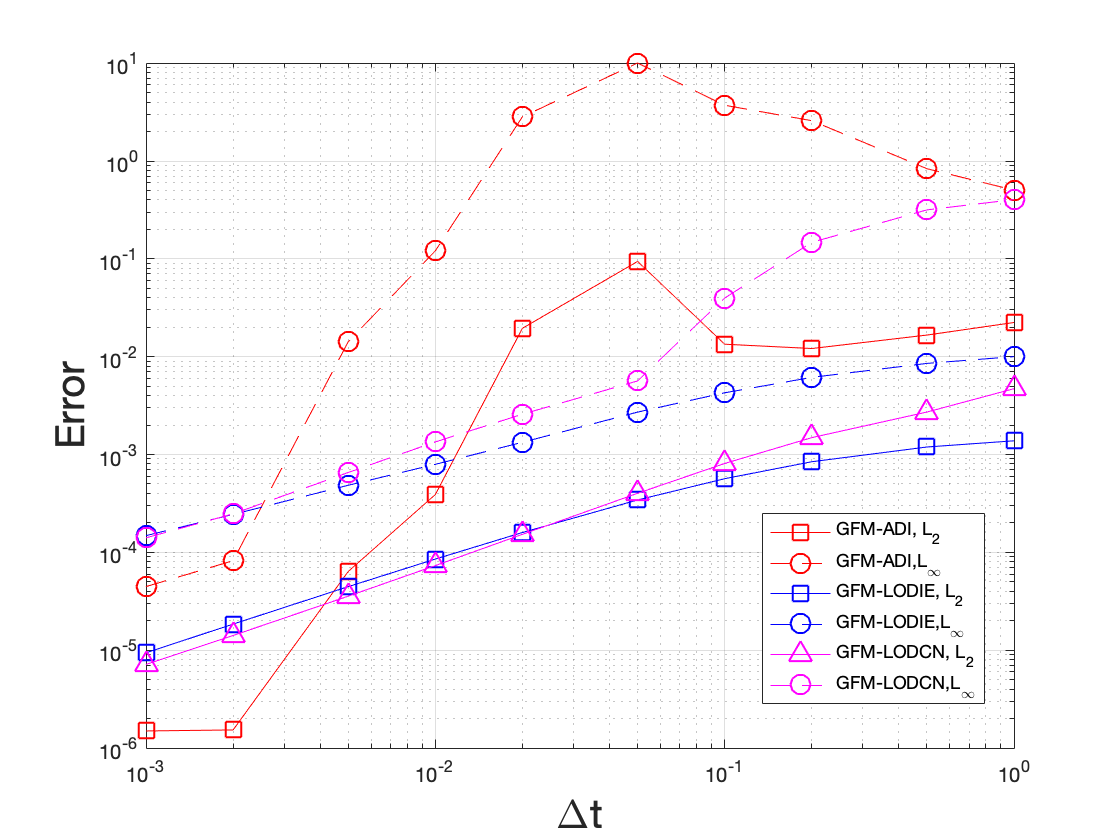
\includegraphics[width=4in]{temp.png}
	\caption{Temporal convergence}
% TODO Have to add ADI methods result 	
\end{figure}
   
\section{Biological applications}

In this section, we focus on exploring the stability and accuracy of GFM-ADI, GFM-LODCN and GFM-LODIE schemes by considering the solvation analysis of real proteins. Even though all of our proposed schemes were found to be stable for the one atom case (Krikwood sphere) for $\Delta t =[0.001,5]$, it is of great interest to see if these schemes are stable for real protein systems. We will compare all three methods in detail for a particular protein system and try to identify the best choice for the time increment $\Delta t $ and the grid spacing $h$ to get the most accurate result within a reasonable amount of time. The optimum $\Delta t$ and $h$ has been used later to calculate the solvation energy of 24 proteins.      

\subsection{Protein Crambin } To validate our proposed schemes with a real protein we have studied the hydrophobic protein Crambin (PDB ID : 1cbn). It is a 46 residue protein homologous to a membrane-active plant toxins \cite{1cbn_paper}. It is found in the seeds of \textit{Crambe abyssinicia} and have local anesthetic activity in a lobster walking leg axon (J. Marquis \cite{1cbn_paper}). We used the MSMS package to generate the molecular surface for this protein using the crystallographic data recored at $130 K$ as reported in \cite{1cbn_paper}. At this step we used the probe radius as $1.4$ the density as $10$ for the MSMS package.
% Table generated by Excel2LaTeX from sheet '1cbn'
\begin{table}[!ht]
\centering
\begin{tabular}{c c c c c }
\hline
%      & \multicolumn{3}{c }{h =1/2}                   \\ \hline
$\Delta t$  & ADI  & GFM-ADI       & GFM-LODCN     & GFM-LODIE     \\ \hline
%0.001 & -302.90138868 & -302.83729044 & -302.03341621 \\ %\hline
%0.005 & -302.90138868 & -302.83729044 & -302.03341621 \\ %\hline
%0.01  & -302.85075766 & -302.68957418 & -301.31096348 \\ %\hline
%0.02  & -302.69227062 & -302.33466174 & -300.06953533 \\ %\hline
%%0.03  & -302.49342491 & -301.93879794 & -298.97743897 \\ \hline
%%0.04  & -302.27488337 & -301.51872505 & -297.97906854 \\ \hline
%0.05  & -302.04538862 & -301.08386563 & -297.04896758 \\ %\hline
%%0.06  & -301.80951214 & -300.64096822 & -296.17267652 \\ \hline
%%0.07  & -301.56994437 & -300.19496277 & -295.34086258 \\ \hline
%%0.08  & -301.32859818 & -299.74929181 & -294.54698251 \\ \hline
%%0.09  & -301.08701698 & -299.30637260 & -293.78618610 \\ \hline
%0.1   & -300.84648128 & -298.86787256 & -293.05472908 \\ %\hline
%0.2   & -298.63624081 & -294.81110682 & -286.88648904 \\ %\hline
%%0.3   & -296.77150162 & -291.23283125 & -282.05981018 \\ \hline
%0.5   & -293.21633440 & -284.83429816 & -274.64462149 \\ %\hline
%0.7   & NaN           & -279.04495504 & -269.01031327 \\ %\hline
%%0.9   & NaN           & -273.75954410 & -264.47533078 \\ \hline
%1     & NaN           & -271.29161057 & -262.50478312 \\ %\hline
%2     & NaN           & -251.54655749 & -248.89416804 \\ %\hline
%%3     & NaN           & -237.49060662 & -240.78175990 \\ \hline
%5     & NaN           & -218.29937773 & -230.91124478 \\\hline
0.001 & -459.5742719854 & -303.00657886   & -303.00154088   & -302.80556740 \\
0.002 & -458.1104685049 & -302.99808443   & -302.98279503   & -302.61375402 \\
0.005 & -452.1116748705 & -302.90138868   & -302.83729044   & -302.03341621   \\
0.01  &    NaN         & -302.85075766   & -302.68957418   & -301.31096348   \\
0.02  &    NaN         & -302.69227062   & -302.33466174   & -300.06953533   \\
0.05  &    NaN          & -302.04538862   & -301.08386563   & -297.04896758   \\
0.1   &    NaN          & -300.84648128   & -298.86787256   & -293.05472908   \\
0.2   &    NaN           & -298.63624081   & -294.81110682   & -286.88648904   \\
0.5   &    NaN          & -293.21633440   & -284.83429816   & -274.64462149   \\
0.7   &   NaN           & NaN             & -279.04495504   & -269.01031327   \\
1     &     NaN         & NaN             & -271.29161057   & -262.50478312   \\
2     &    NaN          & NaN             & -251.54655749   & -248.89416804   \\
5     &    NaN           & NaN             & -218.29937773   & -230.91124478 \\ \hline
\end{tabular}
\caption{Solvation Energy ({\it kcal/mol}) of 1cbn for $h=0.5$ and the ionic strength $I_s= 0.15$}
\label{tab-1cbn}
\end{table}

  For this study at first we reported the solvation energy of 1cbn calculated by all three of our proposed schemes in Table \ref{tab-1cbn}. After calculating electrostatic potential $\phi$, equation (\ref{eq_solvation}) has been discretized further to calculate the solvation energy as, 
 \begin{equation}
 	E_{\rm sol} = \sum_i \sum_j \sum_k Q({x_i,y_j,z_k}) \phi_{RF}(x_i,y_j,z_k)
 \end{equation} 
where $Q$ is the trilinear interpolation of the singular charges $q_i$ at the center of the atoms.  The potential values are obtained by scaling our calculated dimensionless potentials with the constant $0.596163438$ corresponding for the room temperature (300K). In all cases a uniform mesh size $h = 0.5$ and a large stopping time $T$ will be used to ensure that the steady state solution is reached. For the dielectric constant we have used $\epsilon^+=80$ for water as the solvent and $\epsilon ^-=1$ the region in side the protein. The ionic strength has been used as $I_s = 0.15$.
 
Here we tried to identify the value of $\Delta t$ as large as possible without losing the adequate amount accuracy for a real protein like 1cbn. But in Table \ref{tab-1cbn} as we have observed  for $\Delta t > 0.5$, GFM-ADI diverges totally while other two schemes loses significant amount of accuracy. If we consider the solvation energy (around -302 {\it kcal/mol}) for $\Delta t =0.005$ as the most accurate one and compare all other solvation energies in Table \ref{tab-1cbn}, it can be observed that with the increase of $\Delta t$ all three proposed schemes looses accuracy but at a different rate. GFM-ADI scheme is usually more accurate while GFM-LODIE schemes more robust to the larger values of $\Delta t$. The performance of GFM-LODCN is roughly in between the other two schemes in terms of accuracy and stability. To be uniform  with the studies for the other proteins in this paper we have used the optimum value for $\Delta t =0.05$ and $h=0.5$. 
\begin{figure}[!ht]
\begin{center}	
	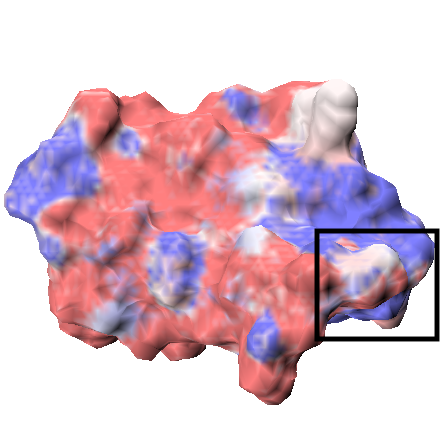
\includegraphics[width=2.1in]{1cbn_gfmadi_front_sq.png}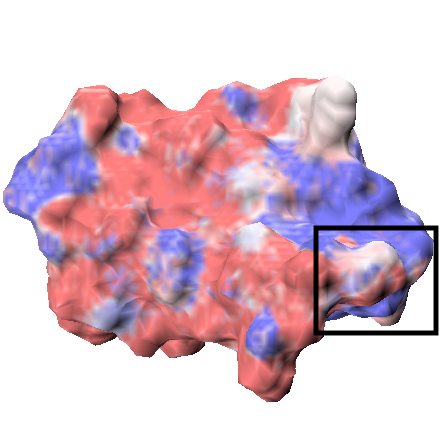
\includegraphics[width=2.1in]{1cbn_gfmlodcn_front_sq.png}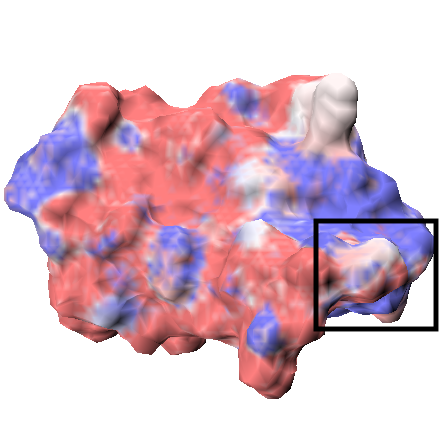
\includegraphics[width=2.1in]{1cbn_gfmlodie_front_sq.png}\\
GFM-ADI front \hskip 0.7in GFM-LODCN front \hskip 0.7in GFM-LODIE front\\
	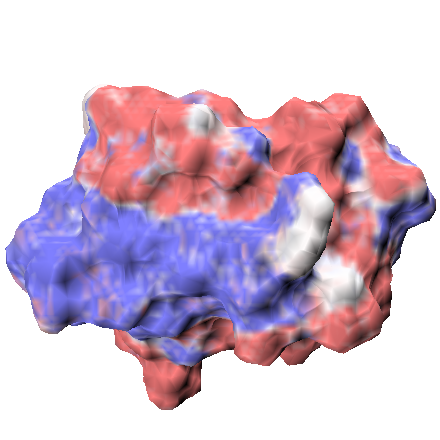
\includegraphics[width=2.1in]{1cbn_gfmlodcn_back.png}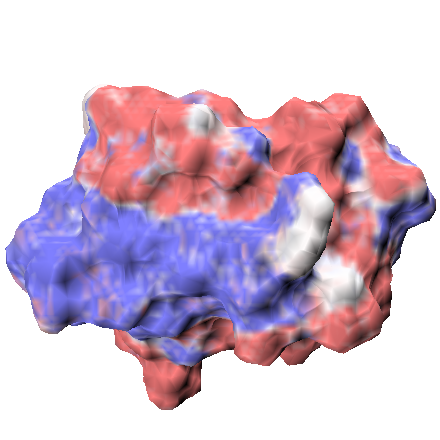
\includegraphics[width=2.1in]{1cbn_gfmlodcn_back.png}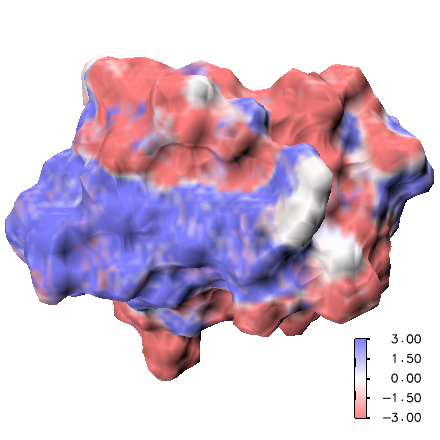
\includegraphics[width=2.1in]{1cbn_gfmlodie_back_scale_1.png}\\
  GFM-ADI back \hskip 0.7in GFM-LODCN back \hskip 0.7in GFM-LODIE back\\
	\caption{Electrostatic potential for 1cbn using $dt = 0.05$ and $h= 0.5$. }
\label{fig_1cbn}
\end{center}
\end{figure}

In Figure \ref{fig_1cbn} we focus on the electrostatic potential on the surface of the protein 1cbn for all three of our prosed schemes.  The difference is not that much noticeable unless we focus in the black squared region of the front side. This shows that, even though there are some differences in solvation energies calculated by the proposed three methods there is no significant difference for the electrostatic potentials for our choice for the optimum values of the parameters.      



\subsection{Solvation energy of 24 proteins}
Next we solved the nonlinear PB equation and computed solvation energy for a collection of 24 proteins as in \cite{Geng2007,Geng2017a}. The dielectric constants , Ionic strength and all other parameters have been set similar to our study for the protein Crambin(1cbn).  
 

\begin{table}[!ht]
\centering
\begin{tabular}{ c c c c c c c c}
\hline
\scriptsize{PDB} & \scriptsize{No. of Atoms}& \scriptsize{rMIB}   &   \scriptsize{ADI}    &  \scriptsize{GFM-ADI}  & \scriptsize{GFM-LODCN} & \scriptsize{GFM-LODIE}\\ \hline
1ajj & 519  & -1139.48 & -1371.10 & -1139.45 & -1139.07 & -1133.06 \\
2erl & 573  & -952.36  & -1165.28 & -952.13  & -951.03  & -945.96  \\
1cbn & 648  & -303.33  & -459.51  & -302.06  & -301.09  & -297.06  \\
1vii & 596  & -902.31  & -1154.67 & -901.78  & -901.36  & -895.15  \\
1fca & 729  & -1204.44 & -1458.16 & -1205.53 & -1205.09 & -1199.33 \\
1bbl & 576  & -988.40  & -1302.49 & -986.15  & -985.72  & -979.60  \\
2pde & 667  & -820.97  & -1018.66 & -819.17  & -819.83  & -813.45  \\
1sh1 & 702  & -753.99  & -999.92  & -751.69  & -751.84  & -745.15  \\
1vjw & 826  & -1241.07 & -1513.17 & -1244.74 & -1243.52 & -1236.67 \\
1uxc & 809  & -1139.25 & -1478.20 & -1138.50 & -1135.22 & -1128.39 \\
1ptq & 795  & -873.32  & -1170.00 & -867.98  & -867.40  & -859.71  \\
1bor & 832  & -853.47  & -1102.40 & -852.49  & -851.24  & -844.68  \\
1fxd & 824  & -3321.39 & -3653.81 & -3321.68 & -3321.34 & -3313.83 \\
1r69 & 997  & -1088.62 & -1419.35 & -1085.45 & -1084.66 & -1076.32 \\
1mbg & 903  & -1353.31 & -1685.70 & -1352.63 & -1351.30 & -1343.68 \\
1bpi & 898  & -1304.37 & -1672.02 & -1301.61 & -1299.86 & -1291.40 \\
1hpt & 858  & -812.49  & -1147.42 & -809.02  & -808.09  & -799.24  \\
451c & 1216 & -1027.21 & -1379.27 & -1023.71 & -1022.61 & -1012.70 \\
1svr & 1435 & -1711.11 & -2257.80 & -1707.87 & -1706.38 & -1693.11 \\
1frd & 1478 & -2862.50 & -3376.35 & -2863.69 & -2863.03 & -2850.42 \\
1a2s & 1272 & -1921.20 & -2292.15 & -1919.28 & -1917.70 & -1907.96 \\
1neq & 1187 & -1731.71 & -2223.08 & -1729.87 & -1728.61 & -1716.47 \\
1a63 & 2065 & -2374.41 & -3149.69 & -2370.80 & -2369.26 & -2350.42 \\
1a7m & 2809 & -2160.34 & -2771.41 & -2155.05 & -2152.48 & -2135.73 \\ \hline
\end{tabular}
\caption{Solvation energies ({\it kcal/mol}) of 24 Proteins considering $\Delta t = 0.001$ for ADI and $\Delta t =0.05$ for GFM-ADI, GFM-LODCN, GFM-LODIE}
\label{tab_24protein}
\end{table}
Solvation energies for all three of our proposed schemes have been compared  with the rMIB and MIB schemes in Table \ref{tab_24protein}. The results from our proposed schemes have been observed to be very close to the results from rMIB and MIB schemes while solving nonlinear PB equation instead of linear PB equation. As we have identified in previous subsections GFM-ADI  appeared to be more accurate than the other two of our proposed schemes and obtained the same level of accuracy as rMIB and MIB schemes. Table \ref{tab_24protein} also confirms that if GFM-ADI fails to converge for any protein then GFM-LODCN or GFM-LOD can also be used since they are more stable and the results are not that much different than GFM-ADI.   
\begin{figure}
	\centering
	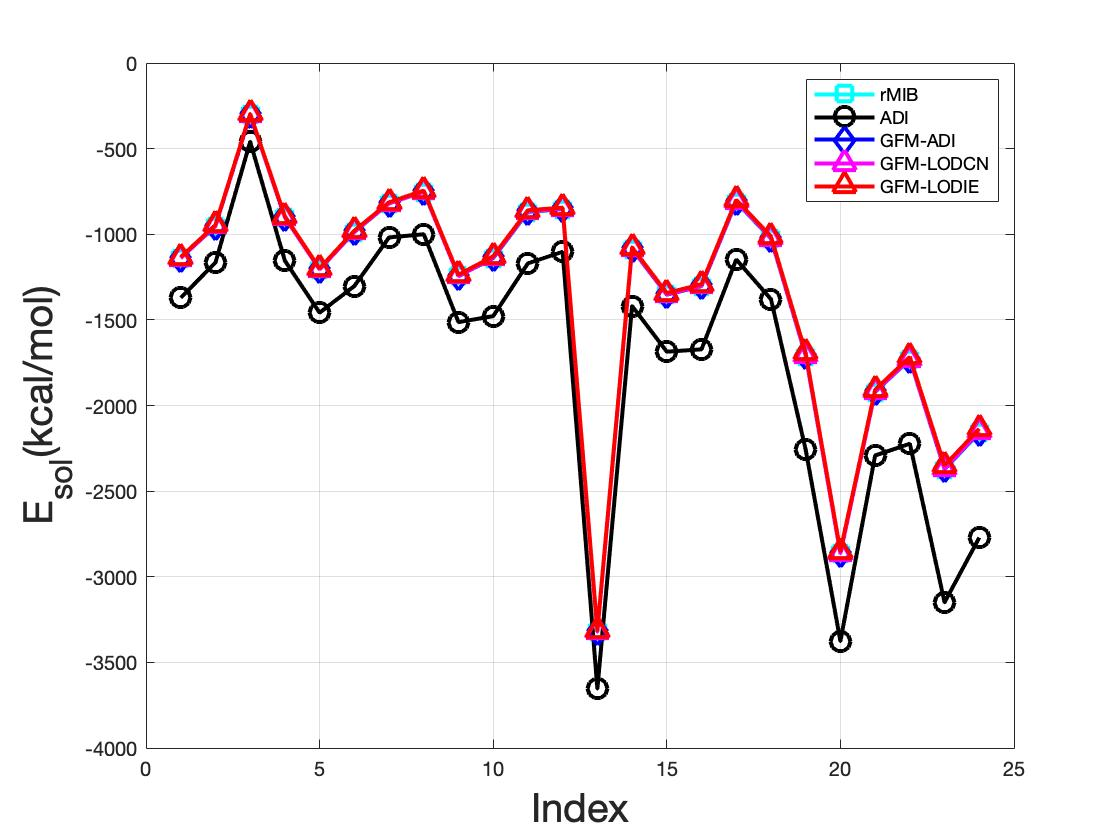
\includegraphics[width=3.2in]{24_energy}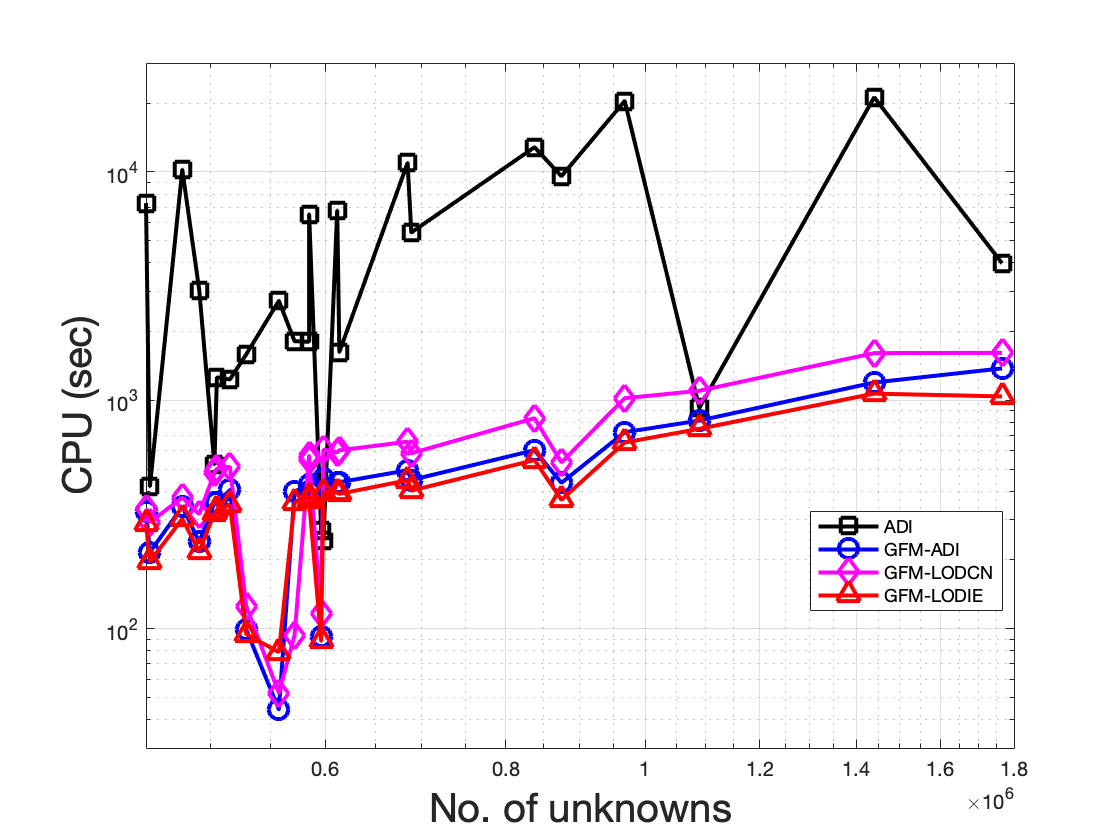
\includegraphics[width=3.2in]{CPU_time}
\caption{Difference in solvation energy(left) and CPU time (right) in solving nonlinear PB eqation for 24 protein. }
\end{figure}

\subsection{Binding energy of 2a9x}

Binding energies play an important role in viral transcription and antiviral drug designs. In particular a better accuracy of the binding energy of the BIV Tat Protein and BIV TAR RNA in HIV viral replication can significantly help in search for the new antiviral drugs that repress the replication by blocking transactivation of viral RNA transcription \cite{Leeper2005}. In this section we will demonstrate the ability of GFM-ADI scheme to compute the binding energy of the BIV Tat Protein and BIV TAR RNA. 

The electrostatic binding free energy can be calculated by the following formula based on the free energy cycle,
\begin{eqnarray}
	E^{\rm AB}_{\rm bind}&=&\Delta G^{\rm AB}_{\rm ele}-\Delta G^{\rm A}_{\rm ele}-\Delta G^{\rm B}_{\rm ele}\label{eq_bind}\nonumber \\
	&=& [E^{\rm AB}_{\rm sol}+E^{\rm AB}_{\rm cou}]-[E^{\rm A}_{\rm sol}+E^{\rm A}_{\rm cou}]-[E^{\rm B}_{\rm sol}+E^{\rm B}_{\rm cou}]
\end{eqnarray}
	
where the free energies of the complex $AB$ and its monomers $A$ and $B$ on the RHS can be calculated using the calculated solvation energies in equation (\ref{eq_Gele}). 
\begin{table}[!ht]
\centering
\begin{tabular}{crrrr}
\hline
$h$ & $E_{\rm sol}^{\rm complex}$ & $E_{\rm sol}^{\rm protein}$ & $E_{\rm sol}^{\rm RNA}$ & $E_{\rm bind}^{\rm complex}$ \\ \hline
\multicolumn{5}{c}{rMIB}  \\ \hline
1   & -5816.38 & -1021.94 & -8893.39 & 383.60 \\
1/2 & -5821.22 & -1025.86 & -8898.54 & 387.84 \\
1/4 & -5823.39 & -1026.27 & -8900.52 & 388.05 \\ \hline
\multicolumn{5}{c}{GFM-ADI}  				  \\ \hline
1   & -5834.10 & -1027.14 & -8915.17 & 392.84 \\
1/2 & -5824.82 & -1025.98 & -8905.59 & 391.38 \\
1/4 & -5841.62 & -1026.40 & -8916.69 & 386.12 \\ \hline
\end{tabular}
\caption{Binding energy of 2a9x}
\label{tab_2a9x}
\end{table}


%    where the calculated solvation energies ($E_{\rm sol}$) will be added with the coulomb energies ($E_{\rm cou}$) to get the free energies ($\Delta G$) for the complex $AB$ and the monomers $A$  and $B$. 

\begin{figure}[!ht]
	\begin{center}
		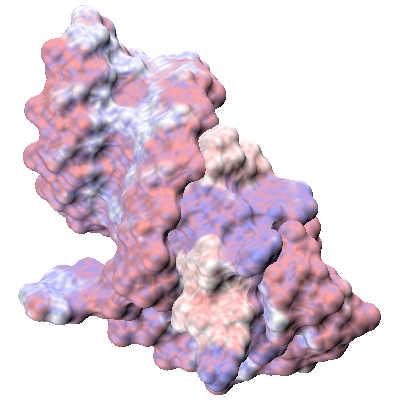
\includegraphics[width=3in]{complex_front.png}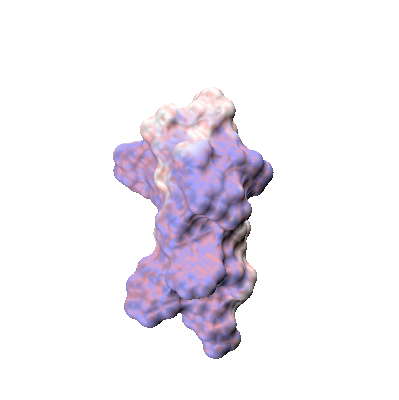
\includegraphics[width=3in]{protein_back.png}\\
		\hskip 0.5in 2a9x complex front\hskip 2.5in 2a9x  protein back\\
		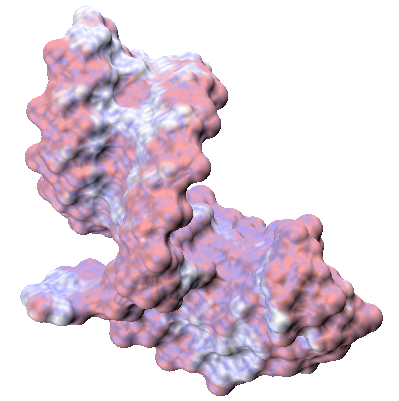
\includegraphics[width=3in]{rna_front.png}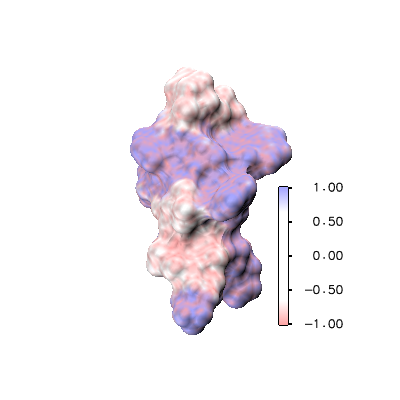
\includegraphics[width=3in]{protein_front_scale_right.png}\\
		\hskip 0.7in 2a9x rna front\hskip 2.8in 2a9x  protein front\\
		\caption{Electrostatic potential for 2a9x using GFM-ADI for $\Delta t = 0.05$ and $h = 0.5$}
	\end{center}
\end{figure}
%todo Have to include the table of binding enrgy

\subsection{Salt effect on the binding affinity}
The nonlinear PB equation is often used to describe the salt effects on the binding of ligands, peptides, and proteins to nucleic acids, membranes, and proteins. In this investigation we have tested the the performance of the proposed GFM-ADI scheme for the evaluation of the salt effect in the protein-protein binding of the complex 1beb and 1emv. Physically, the binding affinity can be quantitatively represented based on the binding-free energies, which reflect the non-specific salt dependence of the formation of macro- molecular complexes. The binding affinity is then calculated as the slope ratio of the salt-dependent binding energy at certain salt strength $I_s$ against the natural logarithm of $I_s$.
The electrostatic binding-free energy can be further split into $E_{\rm cou}(I_s)$'s as the salt-independent parts and $E_{\rm sol}(I_s)$'s as the salt-dependent parts. The variation of the salt-dependent part of the binding-free energy $\Delta E_{\rm bind}(I_s)$ can thus be calculated as the difference in $E_{\rm bind}(I_s)$ for some nonzero salt strength and the zero salt concentration, because the salt independent parts gets simply cancelled. Altogether we have the following formula.\\
\begin{eqnarray}
	\Delta E_{\rm bind}(I_s) &=& E_{\rm bind}(I_s)- E_{\rm bind}(0)\label{eq_del_e_bind} \nonumber\\
						 &=& [E_{\rm sol}^{\rm AB}(I_s)-E_{\rm sol}^{\rm AB}(0)]-[E_{\rm sol}^{\rm A}(I_s)-E_{\rm sol}^{\rm A}(0)]- [E_{\rm sol}^{\rm B}(I_s)-E_{\rm sol}^{\rm A}(0)]\end{eqnarray}
For this study we have used the same model parameters used earlier for 24 proteins. In Figure \ref{fig_salt_effect} we reported the calculated binding free energy with the experimental results.The slope ration or the binding affinity is calculated and reported in Table (\ref{tab_salt_effect}) as in \cite{zhao_pseudo-time-coupled_2011}. The results attained by the Lagrangian formulation linearized PB (LFLPB) model \cite{Zhan_2011} are also given in Table (\ref{tab_salt_effect}) for comparison. For 1beb the binding affinity calculated by GFM-ADI scheme sufficiently close to experimental data and better than LFLPB. For 1emv the results from  GFM-ADI is not as good as those of the LFLPB model but qualitatively it agrees with the experimental observations; that is as the hetero-diemric complex, the binding-free energy increases when the ionic strength is larger. This is probably because the calculation of the binding affinity requires a physical cutoff to obtain two monomers A and B.     	
\begin{table}[!ht]
\begin{tabular}{ccclcrrr}
\hline
\multicolumn{2}{c}{}           & \multicolumn{3}{l}{Charges} & \multicolumn{3}{l}{Slope ratios} \\
Complex                 & PDB  & AB       & A       & B      & Experimental & GFM-ADI & LFLPB   \\ \hline
Lactoglobulin dime(A-B) & 1beb & +26      & +13     & +13    & $-1.62$      & $-1.82$ & $-2.02$ \\ %\hline
E9Dnase-Im9(10)(B-A)    & 1emv & $-3$     & $-8$    & +5     & 2.17         & 0.52    & 2.4     \\ \hline
\end{tabular}
\caption{Comparison of binding affinities of the protein complexes 1emv and 1beb}
\label{tab_salt_effect}
\end{table}



\begin{figure}[!ht]
\begin{center}
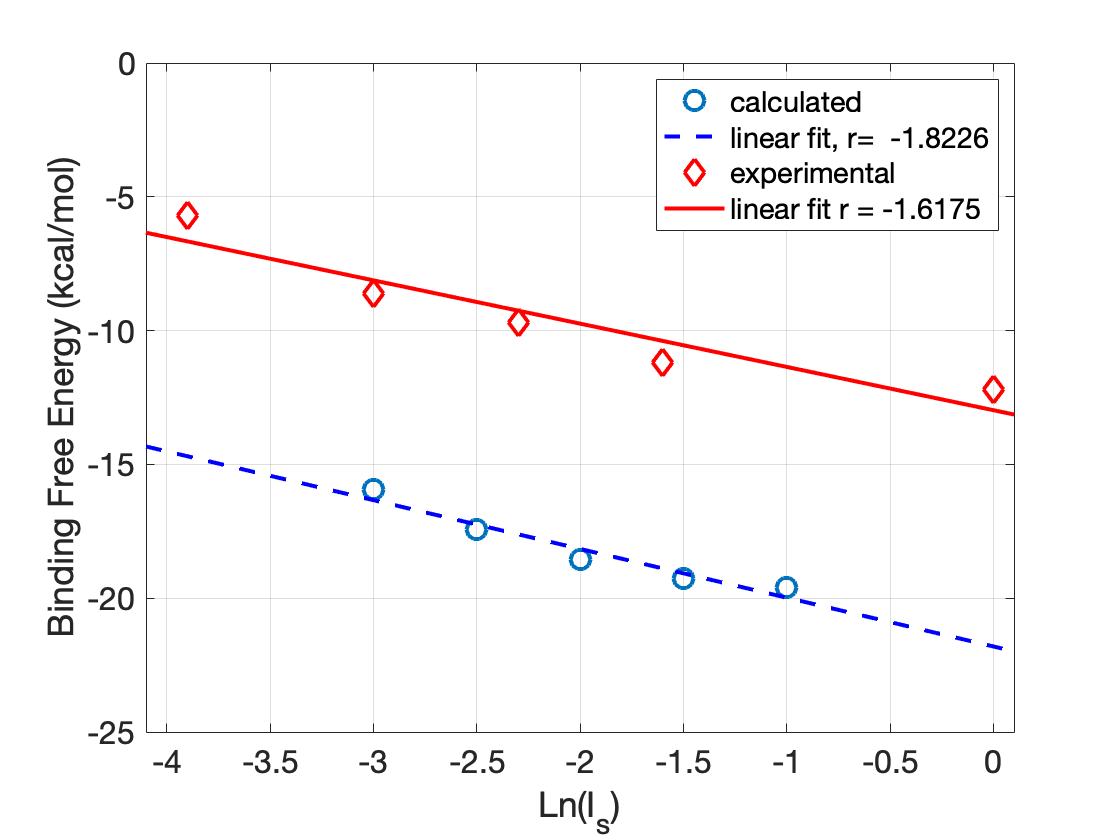
\includegraphics[width =3.2in]{1beb_Tend50_TTol_neg4}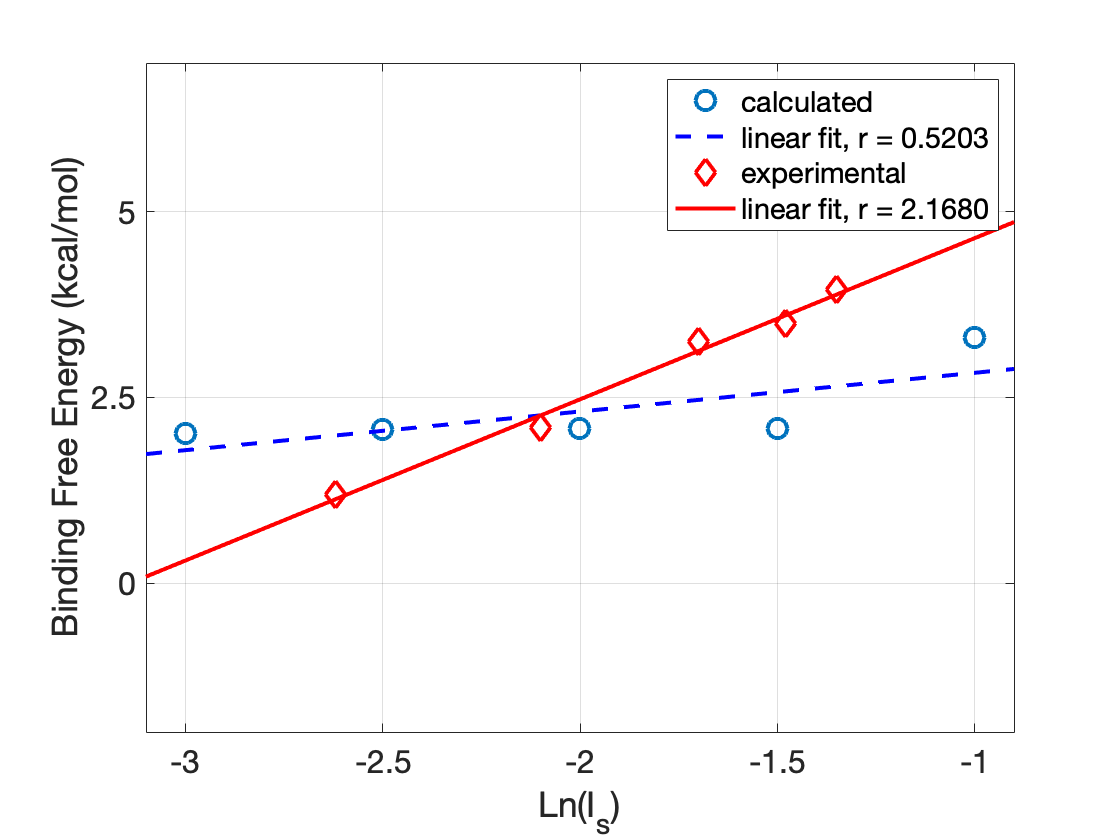
\includegraphics[width =3.2in]{1emv_Tend50_TTol_neg4}\\
1beb \hskip 2.7in 1emv
\end{center}
\caption{The salt dependence of the binding affinities}
\label{fig_salt_effect}
\end{figure}
